\let\negmedspace\undefined
\let\negthickspace\undefined
\documentclass[journal]{IEEEtran}
\usepackage[a5paper, margin=10mm, onecolumn]{geometry}
%\usepackage{lmodern} % Ensure lmodern is loaded for pdflatex
% \usepackage{tfrupee} % Include tfrupee package

\setlength{\headheight}{1cm} % Set the height of the header box
\setlength{\headsep}{0mm}     % Set the distance between the header box and the top of the text

\usepackage{gvv-book}
\usepackage{gvv}
\usepackage{cite}
\usepackage{amsmath,amssymb,amsfonts,amsthm}
\usepackage{algorithm}
\usepackage{algorithmic}
\usepackage{graphicx}
\usepackage{textcomp}
\usepackage{xcolor}
\usepackage{txfonts}
\usepackage{listings}
\usepackage{enumitem}
\usepackage{mathtools}
\usepackage{gensymb}
\usepackage{comment}
\usepackage[breaklinks=true]{hyperref}
\usepackage{tkz-euclide} 
\usepackage{listings}
% \usepackage{gvv}                                        
\def\inputGnumericTable{}                                 
\usepackage[latin1]{inputenc}                                
\usepackage{color}                                            
\usepackage{array}                                            
\usepackage{longtable}                                       
\usepackage{calc}                                             
\usepackage{multirow}                                         
\usepackage{hhline}                                           
\usepackage{ifthen}                                           
\usepackage{lscape}
% \usepackage{algpseudocode}
\begin{document}

\bibliographystyle{IEEEtran}
\vspace{3cm}

\title{NCERT 10.3.2.3.4}
\author{EE24BTECH11053 - S A Aravind Eswar}
% \maketitle
% \newpage
% \bigskip
{\let\newpage\relax\maketitle}

\renewcommand{\thefigure}{\theenumi}
\renewcommand{\thetable}{\theenumi}
\setlength{\intextsep}{10pt} % Space between text and floats

\textbf{Question: } Solve the following equation,
\begin{align}
    5x - 3y = 11\\
    -10x + 6y = -22
\end{align}

\subsection{Theoretical Method:}

If we try to solve the equation, we get infinite number of points as they are coincident.

\subsection{LU decomposition:}

The equations can be written as,
\begin{align}
    \myvec{5 & -3}\vec{x} = 11\\
    \myvec{-10 & 6}\vec{x} = -22
\end{align}

Writing them together,

\begin{align}
    \myvec{5 & -3\\-10 & 6}\vec{x} = \myvec{11\\-22}
\end{align}

which is in the form of

\begin{align}
    A\vec{x} = \vec{b}
\end{align}

We can perform LU decomposition to  find $\vec{x}$

There are multiple way to perform LU decomposition.

\subsubsection{Gaussian Elimination}

    Gaussian Elimination can be written in the following way.

    For a matrix,

    \begin{align}
        A = \myvec{a_{11} & a_{12} & \dots & a_{1n}\\a_{21} & a_{22} & \dots & a_{2n}\\\vdots & \vdots & \vdots & \vdots\\a_{n1} & a_{n2} & \dots & a_{nn}}
    \end{align}

    Given that the diagonal elements aren't zero, we can reduce the first column as,

    \begin{align}
        R_i = R_i - \frac{a_{i1}}{a_{11}}R_1\\
        R_i = R_i - l_{i1}R_1
    \end{align}
    where $i>1$

    Similarly reduing other $n-2$ columns, $A$ is transformed into an upper triangular matrix $U$.

    In general, we can write it as,

    \begin{align}
        R_i = R_i - \frac{a_{ij}}{a_{jj}}R_1\\
        R_i = R_i - l_{i1}R_1
    \end{align}

    $L$ is given by,
    \begin{align}
        L = \myvec{1 & 0 & 0 & \dots & 0\\l_{21} & 1 & 0 & \dots & 0\\ l_{31} & l_{32} & 1 & \dots & 0\\
        \vdots & \vdots & \vdots & \vdots & \vdots\\l_{n1} & l_{n2} & l_{n3} & \dots & 1}
    \end{align}

    Where,

    \begin{align}
        l_{ij} = \frac{a_{ij}}{a_{ii}}
    \end{align}

    \subsubsection{Doolittle's Algorithm}

    Doolittle's algorithm is given by,

    For $U$
    \begin{align}
        \forall &j\\
        i = 0 &\to U_{ij} = A_{ij}\\
        i > 0 &\to U_{ij} = A_{ij} - \sum_{k=0}^{i-1}L_{ik}U_{kj}
    \end{align}
    For $L$

    \begin{align}
        \forall &i\\
        j=0 &\to L_{ij} = \frac{A_{ij}}{U_{jj}}\\
        j>0 &\to L_{ij} = \frac{A_{ij} - \sum_{k=0}^{j-1}L_{ik}U_{kj}}{U_{jj}}
    \end{align}

    After performing LU decomposition, we get,

    \begin{align}
        A = LU
    \end{align}

    where,
    \begin{align}
        L = \myvec{1 & 0\\-2 & 1}\\
        U = \myvec{5 & -3\\0 & 0}
    \end{align}

    Now, we can write the original equation as,

    \begin{align}
        LU\vec{x} = \vec{b}
    \end{align}

    Taking,
    \begin{align}
        U\vec{x} = \vec{y}
    \end{align}

    we get,
    \begin{align}
        L\vec{y} = \vec{b}
    \end{align}

    We can find $\vec{y}$ using forward substitution, giving,
    \begin{align}
        \vec{y} = \myvec{11\\0}
    \end{align}
    Now substituting,
    \begin{align}
        \vec{y} = U\vec{x}
    \end{align}
    We get,
    \begin{align}
        \myvec{5 & -3\\0 & 0}\vec{x} = \myvec{11\\0}
    \end{align}

    As the rank of $U$ is 1, we do not have a unique solution.
    
    As $b_{21}$ is also 0, we can write it as,

    \begin{align}
        \myvec{5 & -3}\vec{x} = 11
    \end{align}

    Implying there are infinite number of solutions for the given pair of equations.

    \begin{figure}[ht]  
        \centering  
        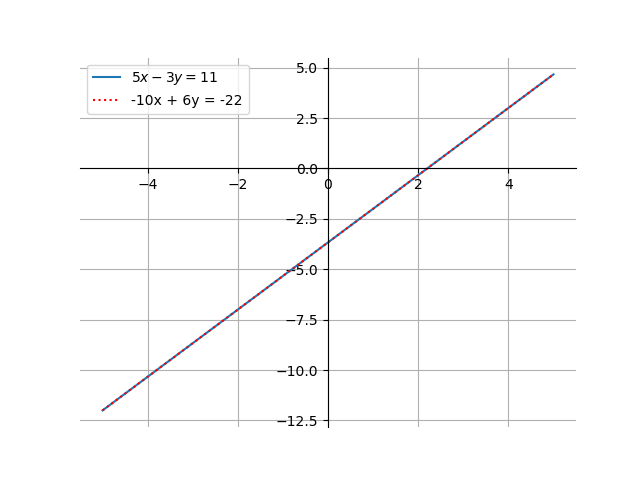
\includegraphics[width=\columnwidth]{figs/fig1.png}  
        \caption{Verification}
        % \columnwidth
    \end{figure}
\end{document}
